\pdfminorversion=7
\documentclass[spanish,aspectratio=1610,xcolor={dvipsnames,table}]{beamer}
\geometry{paperwidth=19.2cm,paperheight=12cm}

\usepackage[utf8]{inputenc}
\usepackage[T1]{fontenc}
\usepackage[spanish,es-nodecimaldot]{babel}
\usepackage{lmodern,amsmath,amssymb,booktabs,array,graphicx,ragged2e,tikz,hyperref}
\usetikzlibrary{arrows.meta,positioning,calc,fit,backgrounds}

\newcommand{\studentname}{Mtro. Martín Jonathan de la Cruz Muñoz}
\newcommand{\studentshort}{M. de la Cruz Munoz}
\newcommand{\studentid}{00874}
\newcommand{\studentemail}{martin.delacruz@campus.iiiepe.edu.mx}
\newcommand{\programname}{Maestría en Enseñanza y Aprendizaje de las Matemáticas}
\newcommand{\programshort}{MAEM}
\newcommand{\coursecode}{PFM02}
\newcommand{\coursename}{Temas selectos de matemáticas I}
\newcommand{\courseperiod}{Ago--Nov 2026 (SD26)}
\newcommand{\institutionname}{IIIEPE}
\newcommand{\iiiepelogo}{img/iiiepe/logo-iiiepe-blanco.png}
\newcommand{\iiiepemark}{img/iiiepe/marca-iiiepe.png}

\definecolor{iiiepeNavy}{HTML}{163B5C}
\definecolor{iiiepeBlue}{HTML}{1F6F9F}
\definecolor{iiiepeAqua}{HTML}{20B7A8}
\definecolor{iiiepeOrange}{HTML}{F28C28}
\definecolor{iiiepePaper}{HTML}{F6F8F7}
\definecolor{iiiepeInk}{HTML}{1E2A32}

\mode<presentation>{
  \usetheme{default}
  \usefonttheme{professionalfonts}
  \setbeamertemplate{navigation symbols}{}
  \setbeamertemplate{blocks}[rounded][shadow=false]
}
\hypersetup{colorlinks=true,urlcolor=iiiepeBlue,linkcolor=iiiepeNavy}
\setbeamercolor{background canvas}{bg=white}
\setbeamercolor{normal text}{fg=iiiepeInk,bg=white}
\setbeamercolor{structure}{fg=iiiepeBlue}
\setbeamercolor{frametitle}{fg=white,bg=iiiepeNavy}
\setbeamercolor{title}{fg=white,bg=iiiepeNavy}
\setbeamercolor{block title}{fg=white,bg=iiiepeBlue}
\setbeamercolor{block body}{fg=iiiepeInk,bg=iiiepePaper}
\setbeamercolor{block title alerted}{fg=white,bg=iiiepeOrange}
\setbeamercolor{block body alerted}{fg=iiiepeInk,bg=iiiepeOrange!10}
\setbeamerfont{title}{size=\Large,series=\bfseries}
\setbeamerfont{frametitle}{size=\fontsize{13}{17}\selectfont,series=\bfseries}
\setbeamerfont{block title}{series=\bfseries}
\setbeamertemplate{itemize item}{\textcolor{iiiepeAqua}{$\blacktriangleright$}}

\newcommand{\localLogo}[1]{\IfFileExists{#1}{\includegraphics[height=0.55cm]{#1}}{\textbf{\institutionname}}}
\setbeamertemplate{frametitle}{
  \nointerlineskip
  \begin{beamercolorbox}[wd=\textwidth,ht=1.0cm,dp=0.2cm,leftskip=0.35cm,rightskip=0.25cm]{frametitle}
    \begin{minipage}[c]{0.72\textwidth}\insertframetitle\end{minipage}\hfill\raisebox{-0.08cm}{\localLogo{\iiiepelogo}}
  \end{beamercolorbox}
  \vspace{-0.04cm}{\color{iiiepeOrange}\rule{\textwidth}{1.3pt}}
}
\setbeamertemplate{footline}{
  \leavevmode\hbox{%
    \begin{beamercolorbox}[wd=.34\paperwidth,ht=2.7ex,dp=1ex,leftskip=1em]{author in head/foot}\color{white}\studentshort\end{beamercolorbox}%
    \begin{beamercolorbox}[wd=.42\paperwidth,ht=2.7ex,dp=1ex,center]{title in head/foot}\color{white}\programshort\ -- \coursecode\ (SD26)\end{beamercolorbox}%
    \begin{beamercolorbox}[wd=.24\paperwidth,ht=2.7ex,dp=1ex,rightskip=1em plus 1fil]{date in head/foot}\color{white}Matrícula \studentid\hfill\insertframenumber/\inserttotalframenumber\end{beamercolorbox}%
  }
}
\setbeamercolor{author in head/foot}{bg=iiiepeNavy}
\setbeamercolor{title in head/foot}{bg=iiiepeBlue}
\setbeamercolor{date in head/foot}{bg=iiiepeNavy}

\title{¿Qué sabemos y cómo lo enseñamos?}
\subtitle{Actividad 1 (Sesión 8) · Retos de Área, Perímetro y Propuesta Canva}
\author{\studentname\ (Matrícula \studentid)}
\institute{\institutionname\ · \programname}
\date{10 de octubre de 2026}

\begin{document}
\begin{frame}[plain]
  \centering
  \vspace{0.5cm}
  \IfFileExists{\iiiepemark}{\includegraphics[height=1.6cm]{\iiiepemark}}{}
  \vspace{0.35cm}
  \begin{beamercolorbox}[sep=10pt,center,rounded=true,wd=0.88\textwidth]{title}
    {\Large\bfseries ¿Qué sabemos y cómo lo enseñamos?}\\[6pt]
    {\small\color{iiiepePaper} Actividad 1 (Sesión 8) · Retos de Área, Perímetro y Propuesta Canva}
  \end{beamercolorbox}
  \vspace{0.45cm}
  {\normalsize\bfseries \studentname}\\
  {\small Matrícula \studentid\ · \coursename\ (\coursecode) · \courseperiod}\\
  {\footnotesize 10 de octubre de 2026}
\end{frame}

\begin{frame}{Propósito de la Sesión 8 y Diagnóstico Inicial}
  \begin{block}{Enfoque del Bloque II: Enseñar desde el desafío}
    Superar la memorización mecánica de fórmulas de área y perímetro mediante retos que exigen explorar casos, modelar, justificar y anticipar dificultades del alumnado.
  \end{block}
  \vspace{0.25cm}
  \begin{columns}[T]
    \column{0.48\textwidth}
      \begin{block}{Dinámica ``Adivina preguntando''}
        \begin{itemize}
          \item Tarjeta en la frente con figura, concepto o fórmula matemática.
          \item Límite de preguntas establecido al lanzar un dado.
          \item Diagnostica precisión conceptual entre magnitudes lineales y superficiales.
        \end{itemize}
      \end{block}
    \column{0.48\textwidth}
      \begin{block}{Ponderación del Curso (Slide 4)}
        \begin{itemize}
          \item Actividades en clase: \textbf{30\,\%}
          \item Reportes de lectura a mano: \textbf{20\,\%}
          \item Exposición final: \textbf{20\,\%}
          \item Exámenes: \textbf{15\,\%} | Dinámicas: \textbf{10\,\%} | Maestro: \textbf{5\,\%}
        \end{itemize}
      \end{block}
  \end{columns}
\end{frame}

\begin{frame}{Reto 1: ¡Construye el jardín más grande! ($P = 24\,\text{m}$)}
  \begin{columns}[T]
    \column{0.52\textwidth}
      \small
      \begin{tabular}{cccc}
        \toprule
        \textbf{Largo $l$} & \textbf{Ancho $a$} & \textbf{Perímetro} & \textbf{Área} \\
        \midrule
        $11\text{ m}$ & $1\text{ m}$ & $24\text{ m}$ & $11\text{ m}^2$ \\
        $10\text{ m}$ & $2\text{ m}$ & $24\text{ m}$ & $20\text{ m}^2$ \\
        $9\text{ m}$  & $3\text{ m}$ & $24\text{ m}$ & $27\text{ m}^2$ \\
        $8\text{ m}$  & $4\text{ m}$ & $24\text{ m}$ & $32\text{ m}^2$ \\
        $7\text{ m}$  & $5\text{ m}$ & $24\text{ m}$ & $35\text{ m}^2$ \\
        \textbf{$6\text{ m}$} & \textbf{$6\text{ m}$} & $24\text{ m}$ & \textbf{$36\text{ m}^2$} \\
        \bottomrule
      \end{tabular}
    \column{0.45\textwidth}
      \begin{block}{Demostración de maximalidad}
        Con $l + a = 12$:
        \[
          A(a) = a(12-a) = 36 - (a-6)^2 \le 36\text{ m}^2
        \]
        El óptimo único ocurre en $a = l = 6\text{ m}$. Hay \textbf{6 diseños enteros} no congruentes.
      \end{block}
      \begin{alertblock}{Pausa reflexiva}
        Error común: excluir el cuadrado como rectángulo o creer que $P$ fijo implica $A$ fija.
      \end{alertblock}
  \end{columns}
\end{frame}

\begin{frame}{Reto 2 y Reto 3: Criterios de Validación y Complejidad}
  \begin{columns}[T]
    \column{0.48\textwidth}
      \begin{block}{Reto 2: El arquitecto ($A=48\text{ m}^2, P=28\text{ m}$)}
        $l\cdot a = 48$ y $l+a = 14 \implies t^2-14t+48=0$:
        \[
          l = 8\text{ m},\quad a = 6\text{ m}.
        \]
        \textbf{Sí es posible.} Enseña al alumno a comprobar afirmaciones de autoridad mediante ecuaciones y contraejemplos.
      \end{block}
    \column{0.48\textwidth}
      \begin{block}{Reto 3: El jardín imposible (pared libre)}
        Con $2a+l=24$ y $A\ge 70\text{ m}^2$:
        \[
          A(a) = 24a - 2a^2 = 72 - 2(a-6)^2
        \]
        Soluciones enteras válidas: $(5,14)\to 70$, $\mathbf{(6,12)\to 72}$, $(7,10)\to 70$. Aumenta la \textbf{complejidad del razonamiento}, no solo el cálculo.
      \end{block}
  \end{columns}
\end{frame}

\begin{frame}{Propuesta Colaborativa en Canva — Equipo 4}
  \begin{columns}[T]
    \column{0.46\textwidth}
      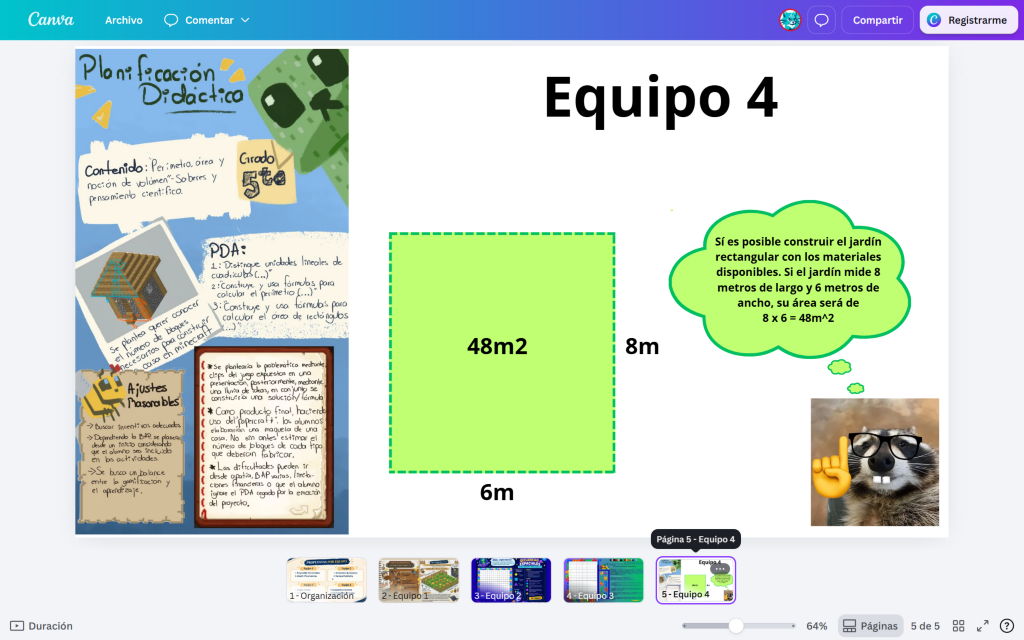
\includegraphics[width=\linewidth]{img/canva/equipo_04_propuesta.png}
      \vspace{0.1cm}
      {\scriptsize Equipo 4: Alejandro Herrera, Christopher de Luna y Jonathan.}
    \column{0.51\textwidth}
      \begin{block}{Planificación Didáctica (5.º Primaria)}
        \begin{itemize}
          \item \textbf{PDA 1--3:} Distingue unidades lineales y cuadráticas; construye fórmulas de perímetro y área.
          \item \textbf{Reto:} Estimar bloques para casa en \textit{Minecraft} y maqueta \textit{papercraft}.
          \item \textbf{Mediación:} Lluvia de ideas guiada y ajustes razonables ante BAP sin dar respuestas directas.
        \end{itemize}
      \end{block}
  \end{columns}
\end{frame}

\end{document}
